% Implementation / Scoping and symtabs
\section{Scoping And Symbol Tables}
\label{sect:impl:scoping_and_symtab}
Scoping was implemented using a simple tree structure consisting of parent- and
child scopes. XQuery only allows new scopes to be defined through the
\verb!enclosedExpr! production rule. This makes it trivial to start a new scope at the
beginning of a \verb!enclosedExpr!, and end the scope and the end of an \verb!enclosedExpr!.
This has been implemented as follows:
\begin{figure}[h!]
\begin{Verbatim}
enclosedExpr : 
    LBRACESi {
        Scope parent = this.currentScope; 
        this.currentScope = new Scope(); 
        this.currentScope.setParent(parent); 
    }
    expr 
    RBRACSi { 
        this.currentScope = this.currentScope.getParent(); 
    }
;
\end{Verbatim}
\caption{Scoping logic embedded in grammar definition}
\end{figure}

Where \verb!this.currentScope! is a reference to the ``current'' scope in this
context. This member variable is initiated with an empty scope when an object
of the parser class is instantiated.
\begin{figure}[h!]
  \centering
    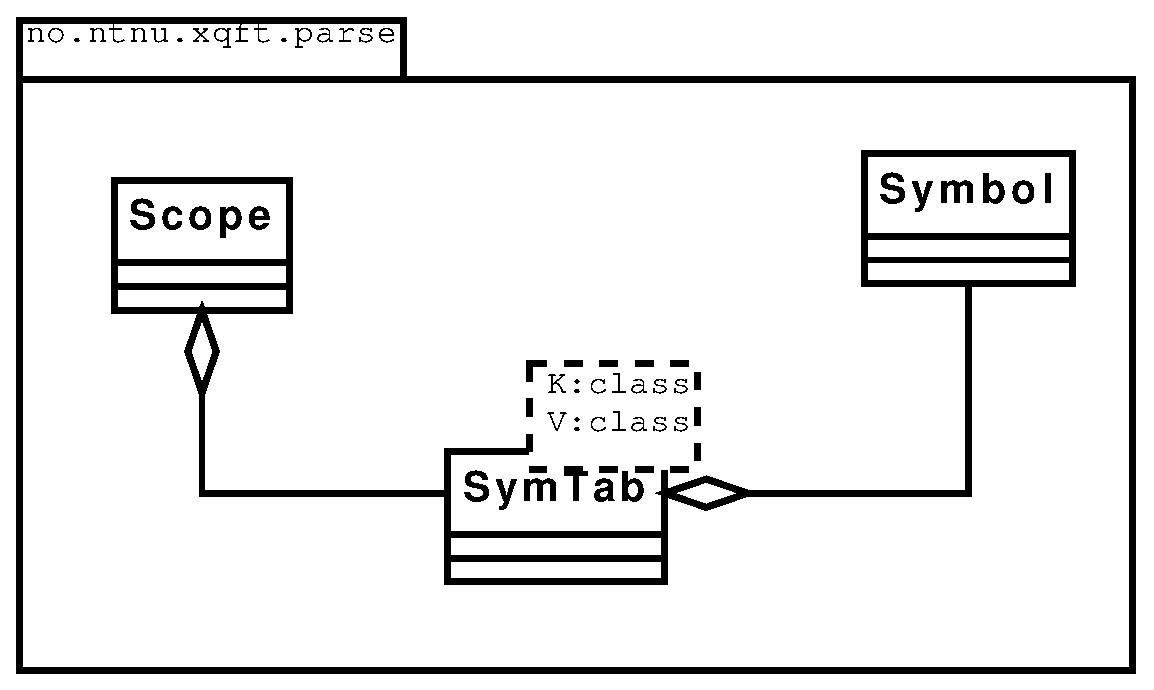
\includegraphics[scale=0.4]{diagrams/uml}
  \caption[Scope and symtab UML diagram]{Simplified UML overview of classes related to
  scope and symbol table}
  \label{fig:scope:uml1}
\end{figure}

The implementation above (which is formatted slightly for brevity) will
automatically build a scope tree as the input is parsed.

The \verb!currentScope! object, which is an object of type \verb!Scope!, holds one reference
to a symbol table. The symbol table, which is a simple subclass of
\verb!java.util.HashMap!, is not capable of performing symbol lookups throughout the
scope tree. This functionality is rather provided by the \verb!Scope! class. The UML diagram
in figure \ref{fig:scope:uml1} illustrates the relationship between the
\verb!Scope!, \verb!SymTab!, and \verb!Symbol! classes.

